
\section{The Distribution of the Scam}
\label{sec:characteristics}


The scams are distributed to the victims via various channels. In this section, we analysis the distribution features in scams.



\subsection{Distribution Channels of Scams}
 
\textbf{Email reports} Email is the most popular bitcoin scam distribution channel. The abuser usually send out the scam information as spamming email.  Table \ref{table:data_detail} shows an example of the content of the scam email. In this example, the abuser field is given as \textit{hs3158@mail.edu.tw}. There are some patterns in the email addresses used by scammers. Overall, there are 56,037 email addresses by 28,229 email domains. One email address can link to many different bitcoin addresses, as shown in figure \ref{fig:email_bitcoin}. The number of reports can be regarded as an index of the influence of the scam. The more an addresses is reported, the more influence the scam has made.

Some of the email addresses are very popular among the reports. Table \ref{table:top10email} shows the top 10 email address reported, together with the number of bitcoin addresses and the number of reports. When analysing the distribution of e-mail addresses, we have collected two datasets, the first one is the complete dataset, with reports range from 16th May, 2017 to 19th Jul, 2020. While the second one is the reports collected to 1st Jan, 2020. By comparing the two datasets, we can find out the change on the distribution of e-mail address used by scammers. Table \ref{table:email_provider} shows the top 10 email provider reported. From this result, we can find out that outlook.com, hotmail.com and yahoo.jp are the most frequently used email service provider in bitcoin scams.



\textbf{Url Information}
There are also some websites that act as a tool for the scammers to reach the victims. Some of the website phishes victims into transferring bitcoin to them. Others might lead the victims to download some ransomwares which can later steal the password of the victim's wallet. Based on our observation, the url information can be devided into three categories. The first one is IP addresses. Some users provide the IP addresses which come from the emails that the scammer send to the victims. The second one is link from big internet service provider such as YouTube\cite{YouTube}, Twitter\cite{twitter}, Instagram\cite{instagram}, there are also link that lead to a telegram\cite{telegram} group. Some of the scammers put their phishing information as a live in video website such as YouTube, or as the form of text message on Twitter. The last one is the link created by the scammers themselves. There are various types of scams related to this type, e.g. typo-squatting the victims into transferring money to the wetsite\cite{xia2020characterizing}. We collected a total of 9,615 urls.
 

\begin{figure}[tbp]
\centerline{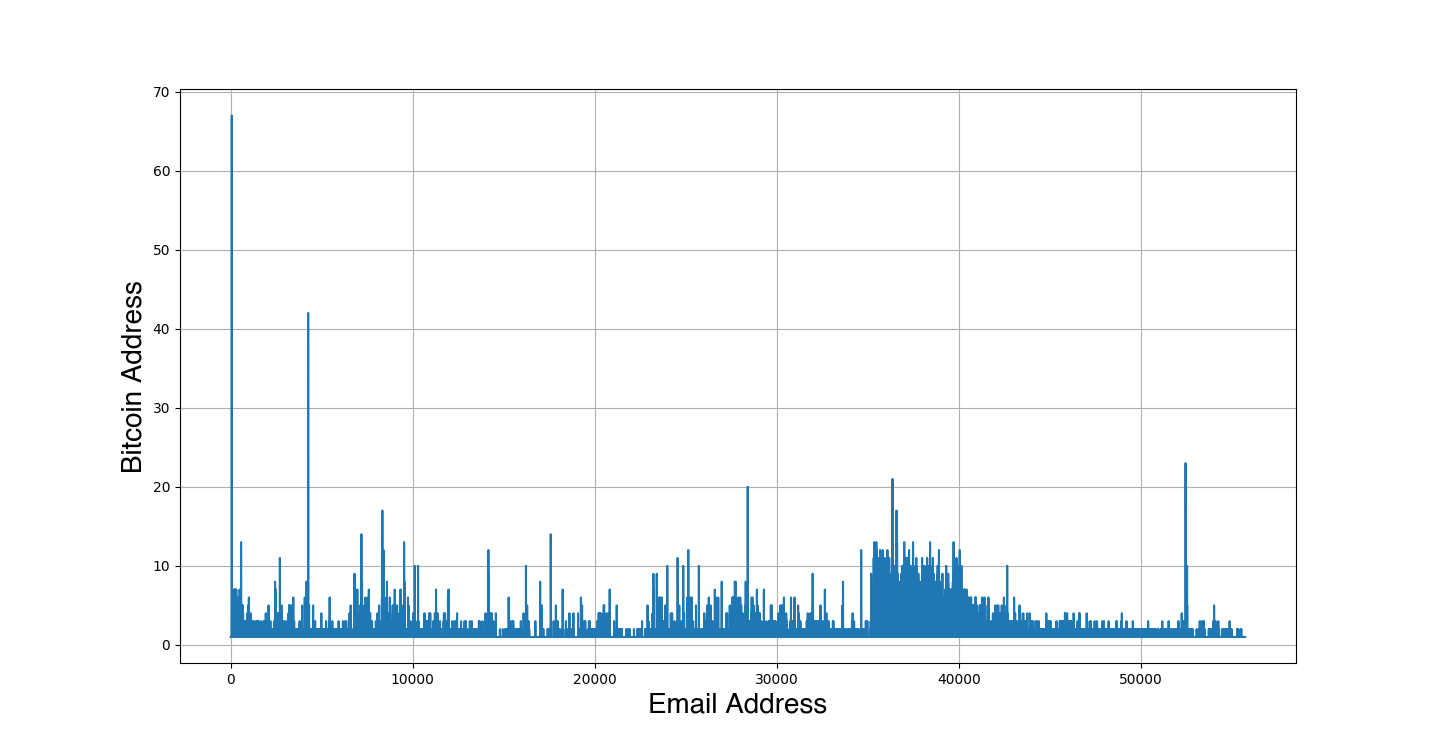
\includegraphics[width=\columnwidth]{images/email_bitcoin.png}}
\caption{The distribution of bitcoin addresses by email addresses}
\label{fig:email_bitcoin}
\end{figure}



\begin{table}[htbp]
\centering
 \caption{The top 10 email addresses\label{table:top10email}}
 \begin{tabular}{lcl}
  \toprule
  Email & Report 1& Report 2 \\
  \midrule
 contract@sqldb.to & 96 & 37\\
 support@mydatabase.to & 81 & 81 \\
 lifeng@01aiche.com & 79 & 79 \\
 info@ednawest.com & 68 & 68\\
 help@sqldb.to & 67 &  \\
 muhstik@protonmail.com & 65 & 65 \\
 olesya.pavlova@thcp.eu& 65 & 60\\
 mateusz@usernet.org & 63 & 63 \\
 admin@hello-database.xyz & 46 & 46\\
 admin@yourdatabase.biz & 36 & 36\\
 %admin@gitsbackup.com &&29\\
  \bottomrule
 \end{tabular}
 
\end{table}


\begin{table}[htbp]
\centering
 \caption{The top 10 email provider\label{table:email_provider}}
 \begin{tabular}{lcl}
  \toprule
  Email & Report 1\footnote{The number of reports till Jul 19,2020 } & Report 2 \footnote{The number of reports till Jan 1,2020}\\
  \midrule
 outlook.com &31061 & 2915 \\
 hotmail.com & 1915&  93 \\
 yahoo.jp & 1149 & 1098 \\
 gmail.com & 704& 307 \\
 protonmail.com & 247&149 \\
 acjeducation.com & 246& --\\
 ortangora.com & 231 & --\\
 yahoo.com & 212&96\\
 nirakobca.com & 198& --\\
 dayukavo.com & 192 & --\\
  \bottomrule
 \end{tabular}
\end{table}



\subsection{Scam Classification}
Table \ref{table:data_detail} also gives a description field. Note that the description is written in various language, as the users in bitcoinabuse come from various districts over the world as shown in figure\ref{fig:country-distribution}. We implemented langid\footnote{github.com/saffsd/langid.py} to filter out the content that are not written in English. We then implemented LDA model to find out the topics among these descriptions provided by the users. Given the coherence value distribution shown in figure\ref{fig:coherence}, we decided to choose 29 as the topic number. After extracting the topic number, we manually grouped the topics into campaigns. The result is shown in the appendix.

There are also abusers who try to escape the spam detection. Figure\ref{fig:special_symbol} gives an example, in this case the abusers use special symbols to escape the detection. Figure\ref{fig:special_font} shows using special font to escape the detection. These emails might affect the accuracy of topic analysis, but as the special symbols used varies in different emails and it is hard to detect and translate this kind of emails, so we ignore these emails.
\begin{figure}[tbp]
\centerline{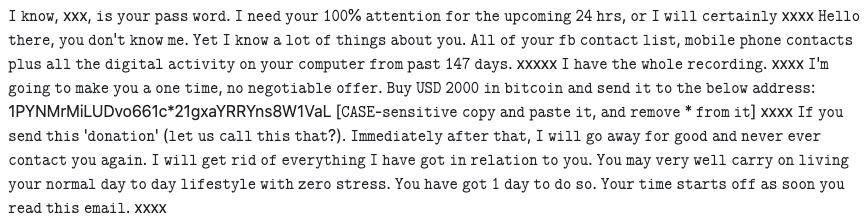
\includegraphics[width=\columnwidth]{images/special_font.png}}
\caption{Special fonts used in emails}
\label{fig:special_font}
\end{figure}

\begin{figure}[tbp]
\centerline{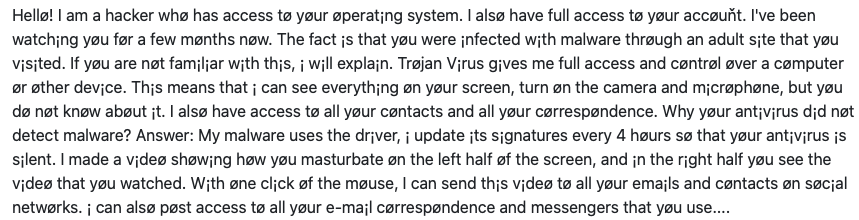
\includegraphics[width=\columnwidth]{images/special_symbol.png}}
\caption{Special symbols used in emails}
\label{fig:special_symbol}
\end{figure}

Figure\ref{fig:word-cloud} shows the word cloud extracted from the description field extracted from all the user reports.
\begin{figure}[tbp]
\centerline{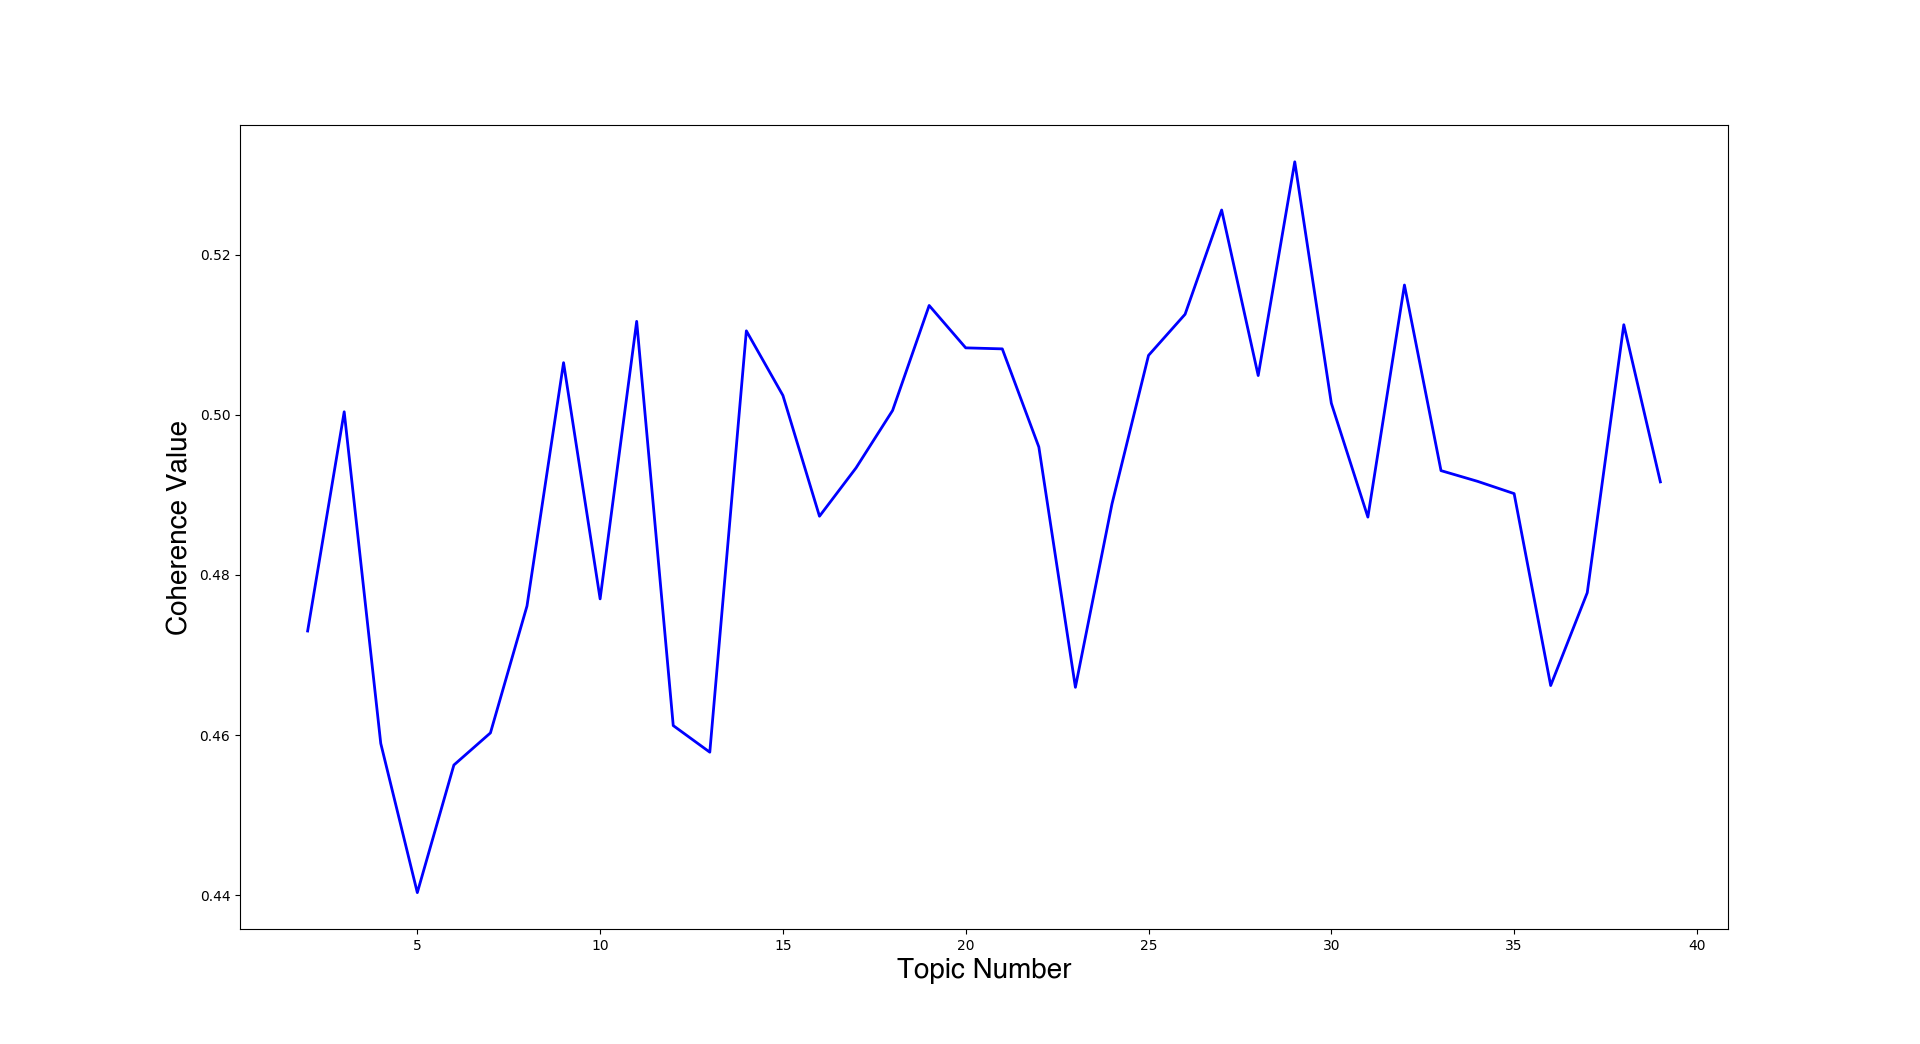
\includegraphics[width=\columnwidth]{images/coherence_graph.png}}
\caption{The coherence value distribution}
\label{fig:coherence}
\end{figure}
\begin{figure}[tbp]
\centerline{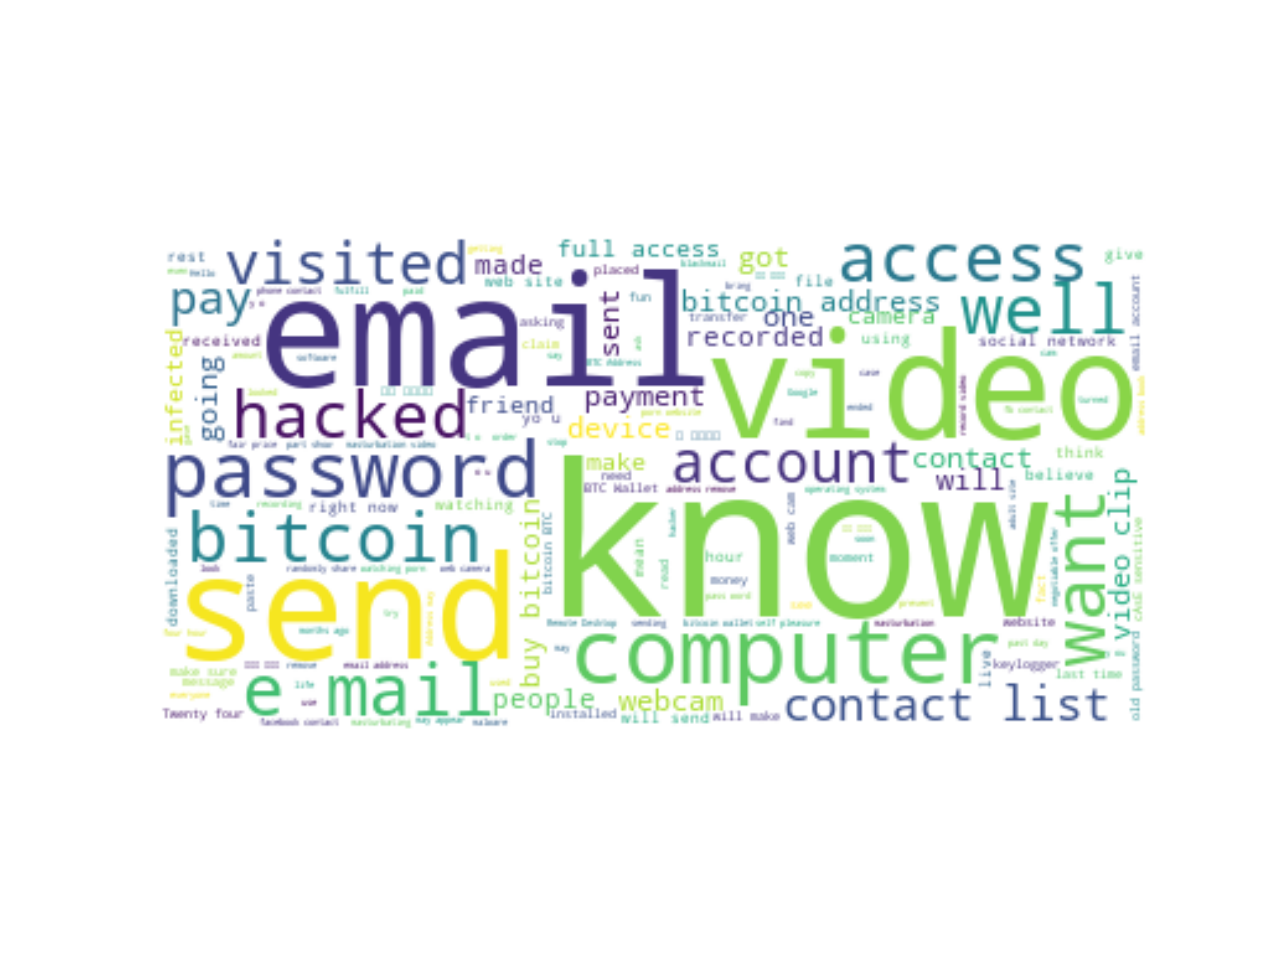
\includegraphics[width=\columnwidth]{images/word_cloud.png}}
\caption{Description Word Cloud.}
\label{fig:word-cloud}
\end{figure}



\noindent\fbox{
\begin{minipage}{0.47\textwidth}{
\textbf{Answer to RQ2}: \textit{Email is one of the most important way to send out scam information for scammers. Here we identified the most frequently used email addresses and most frequently used email service provider. We also analysed the content of these emails.}
}\end{minipage}}



